%%--------------------------------------------------------
%% example.tex
%%
%%--------------------------------------------------------
\documentclass[12pt]{article}
\usepackage{graphicx}
\usepackage[normalem]{ulem}
\usepackage{float}
\usepackage{microtype}
% \usepackage{subfigure} % outdated, use subcaption instead
\usepackage{subcaption}
\usepackage{stackengine}

\usepackage{verbatim} % comment things

\usepackage{amsmath, amssymb, bm, bbm, mathtools}
\usepackage{booktabs} % for professional tables
\usepackage{color}
\usepackage[english]{babel}
\usepackage{times}
\usepackage{nicefrac}

\usepackage{authblk} % author affiliation
\usepackage{xurl} % long url

% Change subfigure numbering style to (a), (b), ...
\renewcommand\thesubfigure{(\alph{subfigure})}

% Apply the format to the sub-figure caption
\captionsetup[subfigure]{labelformat=simple}

% Change equation numbering style to (1), (2), ...
\renewcommand{\theequation}{\arabic{equation}}

% Define new command for equation references
\newcommand{\eqnref}[1]{%
    \ifnum\pdfstrcmp{(}{\unexpanded\expandafter{\@car#1\@nil}}=0
        Equation~\ref{#1}%
    \else
        Equation~(\ref{#1})%
    \fi
}

\newcommand{\theHalgorithm}{\arabic{algorithm}}
\usepackage[linesnumbered,lined,ruled]{algorithm2e}
\SetKwComment{Comment}{$\triangleright$ }{}
% example https://www.overleaf.com/learn/latex/Algorithms#The_algorithm2e_package
\SetKwInOut{Input}{Input}
\SetKwInOut{Output}{Output}
% \SetKwFor{ForEach}{ForEach}{Do}{End}
\SetKwFor{ForEach}{ForEach}{Do}{End}
\SetKwFor{While}{While}{Do}{}
% \SetKwIF{If}{ElseIf}{Else}{If}{Then}{Else If}{Else}{End}
\SetKwIF{If}{ElseIf}{Else}{If}{Then}{Else If}{Else}{}
\SetKwFunction{Return}{\textbf{Return}}
\SetInd{1.5ex}{1.5ex} % Set the indentation width

% --> toc for appendix only
\usepackage[header,page,toc]{appendix}
\usepackage{titletoc}

\definecolor{darkblue}{rgb}{0,0.08,0.45}
\usepackage{hyperref}  % should appear after titletoc

\usepackage{amsthm}
\theoremstyle{plain}
\newtheorem{theorem}{Theorem}[section]
\newtheorem{corollary}[theorem]{Corollary}
\newtheorem{lemma}[theorem]{Lemma}
\newtheorem{proposition}[theorem]{Proposition}

% unnumbered in appendix
\newtheorem*{thm}{Theorem}
\newtheorem*{prop}{Proposition}
\newtheorem*{lma}{Lemma}
\newtheorem*{coro}{Corollary}

\theoremstyle{definition}
% \newtheorem{strategy}{Strategy}[section]
% \renewcommand{\thestrategy}{\Roman{strategy}}
\newtheorem{definition}[theorem]{Definition}
\newtheorem{assumption}[theorem]{Assumption}
\newtheorem{fact}[theorem]{Fact}
\newtheorem{claim}[theorem]{Claim}
\newtheorem{question}[theorem]{Question}

\theoremstyle{remark}
\newtheorem{remark}[theorem]{Remark}

% unnumbered in appendix
\newtheorem*{asmp}{Assumption}

\usepackage{enumitem}

\usepackage[globalcitecopy]{bibunits}
\usepackage{chngcntr}

% Todonotes is useful during development; simply uncomment the next line
%    and comment out the line below the next line to turn off comments
%\usepackage[disable,textsize=normalsize]{todonotes}
\usepackage[disable,textwidth=1.3in,textsize=footnotesize]{todonotes}

% % if you use cleveref..
\usepackage[capitalize,noabbrev]{cleveref}

\usepackage{xcolor}

%%%%%%%%%%%%%%%%%%%%%%%%%%%%%%%%%%%%%%%%%%%%%%%%%%%%%%%%
%%%%%%%%%% ---------- New Commands ---------- %%%%%%%%%%
%%%%%%%%%%%%%%%%%%%%%%%%%%%%%%%%%%%%%%%%%%%%%%%%%%%%%%%%
\usepackage{multirow}
\usepackage{makecell}  % use \multirowcell to handle auto line break in a cell

\usepackage{array}
% Define new column types for left and center alignment with column width as fraction of \textwidth
\newcolumntype{L}[1]{>{\raggedright\let\newline\\\arraybackslash\hspace{0pt}}m{#1\textwidth-2\tabcolsep}}
\newcolumntype{C}[1]{>{\centering\let\newline\\\arraybackslash\hspace{0pt}}m{#1\textwidth-2\tabcolsep}}
\newcolumntype{R}[1]{>{\raggedleft\let\newline\\\arraybackslash\hspace{0pt}}m{#1\textwidth-2\tabcolsep}}

% \newcolumntype{L}[1]{>{\raggedright\arraybackslash}m{#1}}
% \newcolumntype{C}[1]{>{\centering\arraybackslash}m{#1}}


% \newcommand{\ubar}[1]{\text{\b{$#1$}}}
\newcommand{\ubar}[1]{\underline{#1}}

\newcommand{\rulesep}{\unskip\ \vrule\ }

\makeatletter
\newcommand*{\indep}{
    \mathbin{
        \mathpalette{\@indep}{}
    }
}
\newcommand*{\nindep}{
    \mathbin{% The final symbol is a binary math operator
        \mathpalette{\@indep}{\not}% \mathpalette helps for the adaptation of the symbol to the different math styles.
    }
}
\newcommand*{\@indep}[2]{%
    % #1: math style
    % #2: empty or \not
    \sbox0{$#1\perp\m@th$}%        box 0 contains \perp symbol
    \sbox2{$#1=$}%                 box 2 for the height of =
    \sbox4{$#1\vcenter{}$}%        box 4 for the height of the math axis
    \rlap{\copy0}%                 first \perp
    \dimen@=\dimexpr\ht2-\ht4-.2pt\relax
    % The equals symbol is centered around the math axis.
    % The following equations are used to calculate the
    % right shift of the second \perp:
    % [1] ht(equals) - ht(math_axis) = line_width + 0.5 gap
    % [2] right_shift(second_perp) = line_width + gap
    % The line width is approximated by the default line width of 0.4pt
    \kern\dimen@
    {#2}%
    % {\not} in case of \nindep;
    % the braces convert the relational symbol \not to an ordinary
    % math object without additional horizontal spacing.
    \kern\dimen@
    \copy0 %                       second \perp
}
\makeatother

\DeclareMathOperator*{\argmax}{argmax} % thin space, limits underneath in displays
\DeclareMathOperator*{\argmin}{argmin}

\newcommand{\fracpartial}[2]{\frac{\partial #1}{\partial  #2}}

% for creating titles for both main paper and appendix
\makeatletter
\newcommand{\settitle}{\@maketitle}
\makeatother

%% \begin{}\label{bunch of symbols}
% mathbb
\newcommand{\Ebb}{\mathbb{E}}
\newcommand{\Nbb}{\mathbb{N}}
\newcommand{\Rbb}{\mathbb{R}}


% mathbf
\newcommand{\Fbf}{\mathbf{F}}
\newcommand{\Ibf}{\mathbf{I}}
\newcommand{\Kbf}{\mathbf{K}}
\newcommand{\Lbf}{\mathbf{L}}
\newcommand{\Vbf}{\mathbf{V}}
\newcommand{\Zbf}{\mathbf{Z}}

\newcommand{\abf}{\mathbf{a}}
\newcommand{\cbf}{\mathbf{c}}
\newcommand{\fbf}{\mathbf{f}}
\newcommand{\sbf}{\mathbf{s}}
\newcommand{\tbf}{\mathbf{t}}
\newcommand{\ubf}{\mathbf{u}}
\newcommand{\vbf}{\mathbf{v}}
\newcommand{\wbf}{\mathbf{w}}
\newcommand{\xbf}{\mathbf{x}}
\newcommand{\ybf}{\mathbf{y}}
\newcommand{\zbf}{\mathbf{z}}

% boldsymbol
\newcommand{\Kbs}{\boldsymbol{K}}

\newcommand{\abss}{\boldsymbol{a}}
\newcommand{\fbs}{\boldsymbol{f}}
\newcommand{\kbs}{\boldsymbol{k}}
\newcommand{\wbs}{\boldsymbol{w}}
\newcommand{\xbs}{\boldsymbol{x}}
\newcommand{\ybs}{\boldsymbol{y}}
\newcommand{\zbs}{\boldsymbol{z}}

\newcommand{\Phibs}{\boldsymbol{\Phi}}
\newcommand{\Psibs}{\boldsymbol{\Psi}}
\newcommand{\alphabs}{\boldsymbol{\alpha}}
\newcommand{\betabs}{\boldsymbol{\beta}}
\newcommand{\phibs}{\boldsymbol{\phi}}
\newcommand{\xibs}{\boldsymbol{\xi}}
\newcommand{\psibs}{\boldsymbol{\psi}}


% mathcal
\newcommand{\Acal}{\mathcal{A}}
\newcommand{\Dcal}{\mathcal{D}}
\newcommand{\Ecal}{\mathcal{E}}
\newcommand{\Fcal}{\mathcal{F}}
\newcommand{\Gcal}{\mathcal{G}}
\newcommand{\Hcal}{\mathcal{H}}
\newcommand{\Ical}{\mathcal{I}}
\newcommand{\Kcal}{\mathcal{K}}
\newcommand{\Lcal}{\mathcal{L}}
\newcommand{\Ncal}{\mathcal{N}}
\newcommand{\Qcal}{\mathcal{Q}}
\newcommand{\Rcal}{\mathcal{R}}
\newcommand{\Scal}{\mathcal{S}}
\newcommand{\Vcal}{\mathcal{V}}
\newcommand{\Wcal}{\mathcal{W}}
\newcommand{\Xcal}{\mathcal{X}}
\newcommand{\Ycal}{\mathcal{Y}}
\newcommand{\Zcal}{\mathcal{Z}}


\newcommand{\E}{\mathrm{E}}
\newcommand{\Var}{\mathrm{Var}}
\newcommand{\Cov}{\mathrm{Cov}}
\newcommand{\indicator}{\mathbbm{1}}

\usepackage{pifont}
\newcommand{\cmark}{\color{StrokeColorCBGreen} \small \ding{51}}
\newcommand{\xmark}{\color{FontColorCBRed} \scriptsize \ding{56}}

%\end{}

\errorcontextlines=1000  % easier to debug

% For double column
\setlist[enumerate]{leftmargin=*}%
\usepackage{tikz}
\newcommand{\KL}{\textsf{KL}}
\newcommand{\comp}{\mathsf{c}}

\BibLatexMode{%
   \bibliography{template}
}

\begin{document}

\title{Tight Bounds on the Binomial CDF, and the Minimum of i.i.d Binomials, in terms of KL-Divergence}

\author{Xiaohan Zhu\thanks{Department of Statistics, The University of Chicago} \and 
Mesrob I. Ohannessian\thanks{Department of Electrical and Computer Engineering, The University of Illinois at Chicago} \and Nathan Srebro\thanks{Toyota Technological Institute at Chicago}}

% \author{%
%    James Bond%
%    \JamesThanks{Bla bla.}%
%    %
%    \and%
%    %
%    Ford Perfect%
%    \thanks{Bla bla.}%
% }
\date{}
\maketitle


\begin{abstract}
    We provide finite sample upper and lower bounds on the Binomial tail probability which are a direct application of Sanov's theorem. We then use these to obtain high probability upper and lower bounds on the minimum of i.i.d.~Binomial random variables.  Both bounds are finite sample, asymptotically tight, and expressed in terms of the KL-divergence.
\end{abstract}

The purpose of this note is to provide, in a self-contained and concise way, both upper {\em and} lower bounds on the Binomial tail, and through that, on the minimum of i.i.d.~Binomial random variables.  The upper bound on the minimum of i.i.d.~Binomials can be seen as a special case of known uniform concentration guarantees.  Our main purpose here, beyond providing an explicit, simple, and self-contained presentation, is to provide also simple matching {\em lower} bounds.  Such lower bounds can then be used in constructing and analyzing lower bounds for different learning methods and situations. 

% \section{finite sample bound on the binomial CDF}
We first prove a finite sample bound on the Binomial cumulative distribution function (CDF) by using Sanov's theorem. Throughout, all logarithms are base-$2$ and KL divergence is measured in bits.
\begin{lemma}[Binomial tail]
\label{lemma}
    Let $X \sim \frac{1}{n}\textnormal{Bin}(n, p)$ be a scaled Binomial random variable. Then for $a \leq p$,
    % \[
    % \log \mathbb{P}(X \leq a) \in -n \KL(a\Vert p) \pm \left(4\log(n+1) + \left|\log \frac{p}{1-p}\right|\right),
    % \]
    \[
    \log \mathbb{P}(X \leq a) \in -n \KL(a\Vert p) \pm \left(4\log(n+1) + \left[\log \frac{p}{1-p}\right]_+\right),
    \]   where $\KL(\alpha\Vert \beta)$ denotes $\KL(Ber(\alpha)\Vert Ber(\beta)) = \alpha\log\frac{\alpha}{\beta} + (1-\alpha)\log\frac{1-\alpha}{1-\beta}$.
\end{lemma}

\begin{proof}
    We write $X = \frac{1}{n}\sum_{i = 1}^n X_i$, where $X_i \overset{\mathrm{iid}}{\sim} \textnormal{Ber}(p)$, and so $X_1, X_2, \cdots, X_n$ is a sequence of $n$ symbols from the alphabet $\mathcal{X} = \{0,1\}$ with type $(1-X,X)$. Denote the true distribution $Q=\textnormal{Ber}(p)$. 
    
    The upper bound follows directly from Sanov's theorem \citep{TC}:
    \begin{equation}\label{eqn1}
        \log \mathbb{P}(X \leq a) \leq -n \KL(a\Vert p) + 2\log(n+1).
    \end{equation}
    To get a finite sample lower bound, we round $a$ to a multiple of $1/n$.  That is, let $k=\lfloor a n \rfloor$ and $\tilde{a}=k/n$, so that $a-1/n < \tilde{a} \leq a$.
    
    % To get a matching finite sample lower bound, consider $a_n = k_n/n$, for some integer $k_n \in \mathbb{N}$ such that $|a_n - a| \leq 1/n$ and $a_n \leq a$. 
    Let $\mathcal{P}_n = \{(P(0), P(1)): (\frac{0}{n}, \frac{n}{n}),(\frac{1}{n}, \frac{n-1}{n}), \cdots, (\frac{n}{n}, \frac{0}{n}) \}$ be the set of types with denominator $n$, and $E = \{P: P(1) \leq a\}$. Then the type $P_{\tilde{a}} = (1-\tilde{a}, \tilde{a})$ lies in the intersection $E \cap \mathcal{P}_n$.

   Given the type $P \in \mathcal{P}_n$, let $T(P) = \{x \in \mathcal{X}^n: P_x = P\}$ denote the type class of $P$, which is the set of sequences of length $n$ and and type $P$. Then, by adapting equations (11.104) to (11.106) in the lower bound proof of \cite{TC}, we have:
    
    \begin{equation*}
         \begin{split}
        \mathbb{P}(X \leq a) = Q^n(E) &= \sum_{P \in E \cap \mathcal{P}_n} Q^n\left( T \left( P \right) \right)\\
        &\geq Q^n \left(T\left(P_{\tilde{a}}\right)\right)\\
        &\geq \frac{1}{(n+1)^2} 2^{-n\KL(\tilde{a}\Vert p)}.
    \end{split}
    \end{equation*}

    Taking the logarithm on both sides yields:
    \begin{equation}
     \log \mathbb{P}(X \leq a) \geq -2\log(n+1) - n\KL(\tilde{a}\Vert p). \tag{*} \label{*}
    \end{equation}
     
    % Since $a - \tilde{a} < 1/n$, we have $\left|\KL(a\Vert p) - \KL(\tilde{a}\Vert p)\right|= \left|(\tilde{a} - a)\log \frac{p}{1-p} + H(a) - H(\tilde{a}) \right|\\ \leq |\tilde{a} - a| \left| \log \frac{p}{1-p} \right| + \left|H(a) - H(\tilde{a}) \right| \leq \frac{1}{n} \left| \log \frac{p}{1-p} \right| + H(\frac{1}{n}) \leq \frac{1}{n} \left| \log \frac{p}{1-p} \right| + \frac{2\log n}{n} $. 
    
    % Plugging this to the inequality \eqref{*} yields that
    % \begin{align}
    %     \log \mathbb{P}(X \leq a) &\geq -2\log(n+1) - n\KL(\tilde{a}\Vert p)\notag\\
    %     &\geq -2\log(n+1) - \left(n\KL(a\Vert p) + 2\log n + |\log \frac{p}{1-p}| \right)\notag\\
    %     &\geq -n \KL(a\Vert p) - 4\log(n+1) - \left|\log \frac{p}{1-p}\right|.\label{eq:cdflower}
    % \end{align}

        Since $a - \tilde{a} < 1/n$, $H(a) - H(\tilde{a}) < H(\frac{1}{n}) < \frac{2}{n} \log n$. This implies that $\KL(\tilde a\Vert p) - \KL(a\Vert p)= (a-\tilde{a})\log \frac{p}{1-p} + H(a) - H(\tilde{a}) \leq \frac{1}{n} \left[ \log \frac{p}{1-p} \right]_+ + \frac{2}{n} \log n$. Plugging this in the inequality \eqref{*} yields
    \begin{align}
        \log \mathbb{P}(X \leq a) &\geq -2\log(n+1) - n\KL(\tilde{a}\Vert p)\notag\\
        &\geq -2\log(n+1) - \left(n\KL(a\Vert p) + 2\log n + \left[\log \frac{p}{1-p}\right]_+ \right)\notag\\
        &\geq -n \KL(a\Vert p) - 4\log(n+1) - \left[\log \frac{p}{1-p}\right]_+.\label{eq:cdflower}
    \end{align}
    
    The upper bound \eqref{eqn1} and lower bound \eqref{eq:cdflower} together yield the desired result.
\end{proof}


Next, we use the finite sample bound on the Binomial CDF to prove the following concentration bounds of the minimum of i.i.d Binomials in terms of KL divergence.


\iffalse
\begin{theorem}[minimum of i.i.d Binomial]\label{thm1}
    Let $\{X_i\}_{i = 1}^r \overset{\mathrm{iid}}{\sim} \frac{1}{n}\textnormal{Bin}(n, p)$, $Z = \min_{i = 1, \cdots, r} X_i$. Then, with probability $1-\delta$,
    \[
    \KL(Z\Vert p) \in \frac{\log r \pm \left(\log \frac{1}{\delta/2} + 4\log (n+1) + \left[ \log \frac{p}{1-p} \right]_+ \right)}{n}.
    \]
\end{theorem}

\begin{proof}
    Consider any interval $[a,b]$, such that $a\leq b\leq p$. Define the following events:
    \begin{eqnarray*}
        U &=& \{ \KL(Z\Vert p) < \KL(a\Vert p) \}, \\
        L &=& \{ \KL(Z\Vert p) > \KL(b\Vert p) \}, \\
        A &=& \{ Z > a \},\textrm{ and} \\
        B &=& \{ Z < b \}.
    \end{eqnarray*}
    \begin{center}
       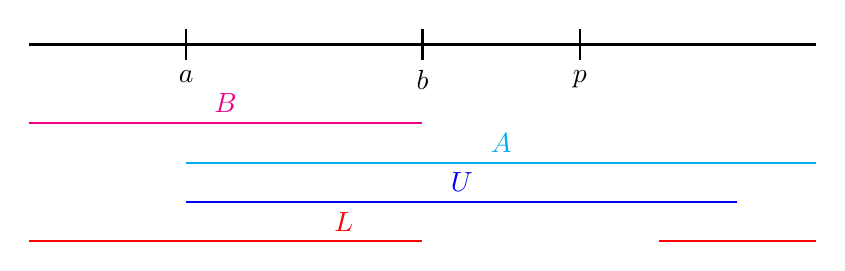
\begin{tikzpicture}
            % Main number line
            \draw[black, thick] (0,0) -- (10,0);
            % Ticks and labels for a, b, and p
            \draw[thick] (2,0.2) -- (2,-0.2) node[below] {$a$};
            \draw[thick] (5,0.2) -- (5,-0.2) node[below] {$b$};
            \draw[thick] (7,0.2) -- (7,-0.2) node[below] {$p$};
            % Magenta line (B)
            \draw[magenta, thick] (0,-1) -- (5,-1) node[midway, above] {$B$};
            % Cyan line (A)
            \draw[cyan, thick] (2,-1.5) -- (10,-1.5) node[midway, above] {$A$};
            % Blue line (U)
            \draw[blue, thick] (2,-2) -- (9,-2) node[midway, above] {$U$};
            % Red lines (L)
            \draw[red, thick] (0,-2.5) -- (5,-2.5);
            \draw[red, thick] (8,-2.5) -- (10,-2.5);
            \node[above] at (4,-2.5) {\textcolor{red}{$L$}};
        \end{tikzpicture}    
    \end{center}
    By the monotonicity of the KL divergence, we have that $B \subseteq L$ and $A \cap B \subseteq U$ (but note that we generally \emph{don't} have $A \subseteq U$). This means that $A \cap B \subseteq U \cap L$, and consequently:
    \[
        \mathbb{P}(U \cap L) \geq  \mathbb{P}(A \cap B)  = 1 - \mathbb{P}(A^\comp) - \mathbb{P}(B^\comp).
    \]
    The theorem will follow from choices of $a$ and $b$ that help bound $\mathbb{P}(A^\comp)$ and $\mathbb{P}(B^\comp)$.
    
    Using the fact that $a \leq p$, along with the union bound and Lemma \ref{lemma}, we have 
    \[
    \mathbb{P}(A^\comp) = \mathbb{P}(Z \leq a) \leq r \cdot\mathbb{P}(X_1 \leq a) \leq r \cdot 2^{-n\KL(a\Vert p) + 4\log (n+1) + \left[ \log \frac{p}{1-p} \right]_+}.
    \]
    Choose $a$ such that $r \cdot 2^{-n\KL(a\Vert p) + 4\log (n+1) + \left[ \log \frac{p}{1-p} \right]_+}=\delta/2$, which gives
    \begin{equation} \label{eq:KLap} 
    \KL(a\Vert p) = \frac{\log r + \log \frac{1}{\delta/2} + 4\log (n+1) + \left[ \log \frac{p}{1-p} \right]_+}{n}.
    \end{equation}
    Thus, by choosing $a$ according to \eqref{eq:KLap}, we get $\mathbb{P}(A^\comp) \leq \frac{\delta}{2}$.

    By the independence of data points, we have:
    \[
    \mathbb{P}(B^\comp) = \mathbb{P}(Z > b) = (1-\mathbb{P}(X_1 \leq b))^r.
    \]
    Using the inequality $\forall x \in [0,1], k > 0: (1-x)^k \leq e^{-kx}$ and Lemma \ref{lemma}, we have
    \[
    (1-\mathbb{P}(X_1 \leq b))^r \leq \exp\left(-r \cdot \mathbb{P}(X_1 \leq b)\right) \leq \exp \left(-r \cdot 2^{-n\KL(b\Vert p) - 4\log (n+1) - \left[ \log \frac{p}{1-p} \right]_+}\right).
    \]
    Choose $b$ such that $\exp \left(-r \cdot 2^{-n\KL(b\Vert p) - 4\log (n+1) - \left[ \log \frac{p}{1-p} \right]_+}\right) = \delta/2 $, which gives
    \begin{equation} \label{eq:KLbp}
    \KL(b\Vert p) = \frac{\log r - \log \ln \frac{1}{\delta/2} - 4\log (n+1) - \left[ \log \frac{p}{1-p} \right]_+}{n}.
    \end{equation}
    Thus, by choosing $b$ according to \eqref{eq:KLbp}, we get $\mathbb{P}(B^\comp) \leq \frac{\delta}{2}$.

    Therefore,
    \begin{equation*}
        \mathbb{P}\Big(\KL(Z\Vert p) \in \big(\KL(b\Vert p), \KL(a\Vert p)\big)\Big) = \mathbb{P}(U\cap L) \geq 1 - \mathbb{P}(A^\comp) - \mathbb{P}(B^\comp) \geq 1-\delta,    
    \end{equation*}
    with $\KL(a\Vert p)$ and $\KL(b\Vert p)$ as in \eqref{eq:KLap} and \eqref{eq:KLbp} respectively. The theorem follows by widening this interval, to get a symmetric expression.
\end{proof}
\fi

\iffalse
% Previous version
\begin{theorem}[minimum of i.i.d Binomial]\label{thm1}
    Let $\{X_i\}_{i = 1}^r \overset{\mathrm{iid}}{\sim} \frac{1}{n}\textnormal{Bin}(n, p)$, $Z = \min_{i = 1, \cdots, r} X_i$. Assume that $Z \leq p$, then with probability $1-\delta$,
    \[
    \KL(Z\Vert p) \in \frac{\log r \pm \left(\log \frac{1}{\delta/2} + 4\log (n+1) + \left[ \log \frac{p}{1-p} \right]_+ \right)}{n}.
    \]
\end{theorem}

\begin{proof}
    Consider some $a \leq p$, with the union bound and Lemma \ref{lemma}, we have 
    \[
    \mathbb{P}(Z \leq a) \leq r \cdot\mathbb{P}(X_1 \leq a) \leq r \cdot 2^{-n\KL(a\Vert p) + 4\log (n+1) + \left[ \log \frac{p}{1-p} \right]_+}.
    \]
    Set the right hand side to be $\delta/2$ such that $\delta/2 = r \cdot 2^{-n\KL(a\Vert p) + 4\log (n+1) + \left[ \log \frac{p}{1-p} \right]_+}$, which gives
    \[
    \KL(a\Vert p) = \frac{\log r + \log \frac{1}{\delta/2} + 4\log (n+1) + \left[ \log \frac{p}{1-p} \right]_+}{n}.
    \]
    Therefore, with probability $1-\delta/2$, we have $Z \geq a$ with $\KL(a\Vert p) = \frac{\log r + \log \frac{1}{\delta/2} + 4\log (n+1) +\left[ \log \frac{p}{1-p} \right]_+}{n}$. Then since $Z \leq p$, by the monotonicity of KL divergence, with probability $1-\delta/2$, we have 
    \begin{equation}
      \KL(Z\Vert p) \leq \KL(a\Vert p) = \frac{\log r + \log \frac{1}{\delta/2} + 4\log (n+1) + \left[ \log \frac{p}{1-p} \right]_+}{n}, 
    \end{equation}
    which proves the upper bound.

    On the other hand, consider some $a' \leq p$, by the independence of data points, $\mathbb{P}(Z \leq a') = 1 -(1-\mathbb{P}(X_1 \leq a'))^r$. Using the inequality $\forall x \in [0,1], k > 0: (1-x)^k \leq e^{-kx}$ and Lemma \ref{lemma}, we have $(1-\mathbb{P}(X_1 \leq a'))^r \leq e^{-r \cdot \mathbb{P}(X_1 \leq a')} \leq e^{-r \cdot 2^{-n\KL(a'\Vert p) - 4\log (n+1) - \left[ \log \frac{p}{1-p} \right]_+}}$. Set the right hand side to be $\delta/2$ such that $\delta/2 = e^{-r \cdot 2^{-n\KL(a'\Vert p) - 4\log (n+1) - \left[ \log \frac{p}{1-p} \right]_+}}$, which gives
    \[
    \KL(a'\Vert p) = \frac{\log r - \log \ln \frac{1}{\delta/2} - 4\log (n+1) - \left[ \log \frac{p}{1-p} \right]_+}{n}.
    \]
    Therefore, with probability $1-\delta/2$, we have $Z \leq a'$ with $\KL(a'\Vert p) = \frac{\log r - \log \ln \frac{1}{\delta/2} - 4\log (n+1) - \left[ \log \frac{p}{1-p} \right]_+}{n}$. Then by the monotonicity of KL divergence, with probability $1-\delta/2$, we have
    \begin{equation}
        \KL(Z\Vert p) \geq \KL(a'\Vert p) = \frac{\log r - \log \ln \frac{1}{\delta/2} - 4\log (n+1) - \left[ \log \frac{p}{1-p} \right]_+}{n},
    \end{equation}
    which proves the lower bound.

    Combining the two events with union bound, we prove the desired concentration bound of minimum of i.i.d Binomial random variables. 
\end{proof}
\fi

\begin{theorem}[minimum of i.i.d Binomial]\label{thm1}
    Let $\{X_i\}_{i = 1}^r \overset{\mathrm{iid}}{\sim} \frac{1}{n}\textnormal{Bin}(n, p)$, $Z = \min_{i = 1, \cdots, r} X_i$. Given fixed confidence parameter $\delta \in (0,1)$, let $\Delta(\delta, p, n) = \log \frac{1}{\delta/2} + 4\log (n+1) + \left[ \log \frac{p}{1-p} \right]_+ $. If $\Delta(\delta, p, n) < \log r$, then with probability $1-\delta$, we have
    \[
    Z < p \text{, and } \KL(Z\Vert p) \in \frac{\log r \pm \Delta(\delta, p, n)}{n},
    \]
    except that if $\KL(0 \Vert p) < \frac{\log r -\Delta(\delta, p, n)}{n}$, then with probability $1-\delta$, $Z = 0$.
\end{theorem}

\begin{proof}
    Consider any interval $[a,b]$, such that $a\leq b< p$. Define the following events:
    \begin{eqnarray*}
        U &=& \{ \KL(Z\Vert p) \leq \KL(a\Vert p) \}, \\
        L &=& \{ \KL(Z\Vert p) \geq \KL(b\Vert p) \}, \\
        A &=& \{ Z \geq a \},\textrm{ and} \\
        B &=& \{ Z \leq b \}.
    \end{eqnarray*}
    \begin{center}
       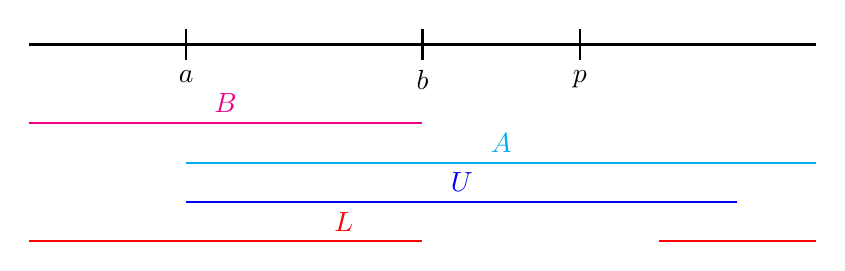
\begin{tikzpicture}
            % Main number line
            \draw[black, thick] (0,0) -- (10,0);
            % Ticks and labels for a, b, and p
            \draw[thick] (2,0.2) -- (2,-0.2) node[below] {$a$};
            \draw[thick] (5,0.2) -- (5,-0.2) node[below] {$b$};
            \draw[thick] (7,0.2) -- (7,-0.2) node[below] {$p$};
            % Magenta line (B)
            \draw[magenta, thick] (0,-1) -- (5,-1) node[midway, above] {$B$};
            % Cyan line (A)
            \draw[cyan, thick] (2,-1.5) -- (10,-1.5) node[midway, above] {$A$};
            % Blue line (U)
            \draw[blue, thick] (2,-2) -- (9,-2) node[midway, above] {$U$};
            % Red lines (L)
            \draw[red, thick] (0,-2.5) -- (5,-2.5);
            \draw[red, thick] (8,-2.5) -- (10,-2.5);
            \node[above] at (4,-2.5) {\textcolor{red}{$L$}};
        \end{tikzpicture}    
    \end{center}
    By the monotonicity of the KL divergence, we have that $B \subseteq L$ and $A \cap B \subseteq U$ (but note that we generally \emph{don't} have $A \subseteq U$). This means that $A \cap B \subseteq U \cap L$, and consequently:
    \[
        \mathbb{P}(U \cap L) \geq  \mathbb{P}(A \cap B)  = 1 - \mathbb{P}(A^\comp) - \mathbb{P}(B^\comp).
    \]
    The theorem will follow from choices of $a$ and $b$ that help bound $\mathbb{P}(A^\comp)$ and $\mathbb{P}(B^\comp)$.
    
    Using the fact that $a<p$, along with the union bound and Lemma \ref{lemma}, we have 
    \[
    \mathbb{P}(A^\comp) =\mathbb{P}(Z < a) \leq \mathbb{P}(Z \leq a) \leq r \cdot\mathbb{P}(X_1 \leq a) \leq r \cdot 2^{-n\KL(a\Vert p) + 4\log (n+1) + \left[ \log \frac{p}{1-p} \right]_+}.
    \]
    Suppose $\KL(0\Vert p) \geq \frac{\log r + \Delta(\delta, p, n)}{n}$. Since $\KL(p\Vert p) = 0$, and KL is continuous by its first argument, by intermediate value theorem, we can choose $0 \leq a <p$ such that
    \begin{equation} \label{eq:KLap} 
    \begin{split}
    \KL(a\Vert p)  &= \frac{\log r + \Delta(\delta, p, n)}{n}\\
    &= \frac{\log r + \log \frac{1}{\delta/2} + 4\log (n+1) + \left[ \log \frac{p}{1-p} \right]_+}{n},
    \end{split}
    \end{equation}
     which gives $r \cdot 2^{-n\KL(a\Vert p) + 4\log (n+1) + \left[ \log \frac{p}{1-p} \right]_+}=\delta/2$.
    Thus, by choosing $0 \leq a < p$ according to \eqref{eq:KLap}, we get $\mathbb{P}(A^\comp) \leq \frac{\delta}{2}$.
    
    If $\KL(0\Vert p) < \frac{\log r + \Delta(\delta, p, n)}{n}$, in other words, there is no $0 \leq a < p$ satisfying \eqref{eq:KLap}, then take $a = 0$. And in this case, the upper bound of the theorem trivially holds for any $Z < p$ because
    \begin{align*}
        \mathbb{P}\left(\KL(b \Vert p) \leq \KL(Z\Vert p) \leq \KL(0 \Vert p) < \frac{\log r + \Delta(\delta, p, n)}{n}\right) &\geq \mathbb{P}(0 \leq Z \leq b)
        = 1 - \mathbb{P}(Z > b).
    \end{align*}

    On the other hand, by the independence of data points, we have:
    \begin{equation}\label{eq:indep}
    \mathbb{P}(B^\comp) = \mathbb{P}(Z > b) = (1-\mathbb{P}(X_1 \leq b))^r.
    \end{equation}
    Using the inequality $\forall x \in [0,1], k > 0: (1-x)^k \leq e^{-kx}$ and Lemma \ref{lemma}, we have
    \begin{equation}\label{eq:expbd}
    (1-\mathbb{P}(X_1 \leq b))^r \leq \exp\left(-r \cdot \mathbb{P}(X_1 \leq b)\right) \leq \exp \left(-r \cdot 2^{-n\KL(b\Vert p) - 4\log (n+1) - \left[ \log \frac{p}{1-p} \right]_+}\right).
    \end{equation}
    Suppose $\KL(0\Vert p) \geq \frac{\log r - \log \ln \frac{1}{\delta/2} - 4\log (n+1) - \left[ \log \frac{p}{1-p} \right]_+}{n}$, again by the intermediate value theorem, we can choose $0 \leq b < p$ such that 
    \begin{equation} \label{eq:KLbp}
    \KL(b\Vert p) = \frac{\log r - \log \ln \frac{1}{\delta/2} - 4\log (n+1) - \left[ \log \frac{p}{1-p} \right]_+}{n}, 
    \end{equation}
    which gives $\exp \left(-r \cdot 2^{-n\KL(b\Vert p) - 4\log (n+1) - \left[ \log \frac{p}{1-p} \right]_+}\right) = \delta/2$.
    Thus, by choosing $0 \leq b <p$ according to \eqref{eq:KLbp}, we get $\mathbb{P}(B^\comp) \leq \frac{\delta}{2}$.

    If $\KL(0\Vert p) < \frac{\log r - \log \ln \frac{1}{\delta/2} - 4\log (n+1) - \left[ \log \frac{p}{1-p} \right]_+}{n}$, in other words, there is no $0\leq b < p$ satisfying \eqref{eq:KLbp}, then by combining \eqref{eq:indep} and \eqref{eq:expbd},
    \[
        \mathbb{P}(Z > 0)\leq \exp \left(-r \cdot 2^{-n\KL(0\Vert p) - 4\log (n+1) - \left[ \log \frac{p}{1-p} \right]_+}\right)
        \leq \frac{\delta}{2}.
    \]
    So in this case, we have with probability $\geq \frac{\delta}{2} > 1 - \delta$, $Z = 0$.

    Therefore, by choosing $a$ and $b$ as above, we get
    \begin{equation*}
        \mathbb{P}\Big(\KL(Z\Vert p) \in \big(\KL(b\Vert p), \KL(a\Vert p)\big)\Big) = \mathbb{P}(U\cap L) \geq 1 - \mathbb{P}(A^\comp) - \mathbb{P}(B^\comp) \geq 1-\delta,    
    \end{equation*}
    with $\KL(a\Vert p)$ and $\KL(b\Vert p)$ as in \eqref{eq:KLap} and \eqref{eq:KLbp} respectively. Except that if $\KL(0\Vert p) < \frac{\log r - \Delta(\delta, p, n)}{n}$, then with probability $> 1 - \delta$, $Z = 0$.
 
    The theorem follows by widening this interval, to get a symmetric expression.
\end{proof}

\begin{remark}
    The term $\left[\log \frac{p}{1-p}\right]_+$ is not actually needed in the upper bounds in Lemma \ref{lemma} and  Theorem \ref{thm1}, and is included in the Theorem statement only for the sake of a symmetric and concise statement.
\end{remark}

\begin{remark}
The upper bound in Theorem \ref{thm1} does not rely on $X_i$ being independent, nor even identically distributed. In fact, as long as $X_i \sim \frac{1}{n}\textnormal{Bin}(n, p_i)$ marginally with $p_i \geq p$, the upper bound still holds.  This union-bound based upper bound can be viewed as a (one sided) concentration guarantee, thinking of each $X_i$ as an empirical average with mean $p$, and ensuring that all $n$ empirical measurements are close to their expectation (or rather, not much smaller than their expectation).  In a machine learning context, $X_i$ would correspond to the empirical error of predictor $i$, with population error $p$ (or in the more general non-identically-distributed case, with population error $p_i\geq p$).  Viewed this way, the upper bound in Theorem \ref{thm1} is a special case\footnote{Theorem \ref{thm1} is a special case where we take a discrete uniform prior over the $r$ predictors, and are concerned only with point-mass posteriors.} of the PAC-Bayes bound as presented by \citet[][Equation (4)]{mcallester2003simplified} following \citet{langford2001bounds}.  The upper bound is thus similar to, but slightly tighter than, common concentration guarantees based on a similar union-bound argument, but relying on the Hoeffding and Bernstein bounds on the Binomial CDF instead of the KL-based bound of Lemma \ref{lemma}.  Theorem \ref{thm1} shows the KL-based bound is tight, and provides a simple matching lower bound.

    
    % It is worth mentioning that the upper bound of $\KL(Z\Vert p)$ proved in Theorem 1 is a special case of the concentration inequality we use for $\textnormal{MDL}_1$ agnostic analysis: $\textnormal{ KL}(L_S(h) \Vert  L(h)) \leq \frac{-\log \pi(h) + O(\log \frac{n}{\delta})}{n}$, where $\pi$ is a prior over $h$, $L_S(h) = \frac{1}{n} \sum_{j = 1}^n \mathbbm{1}_{h(x_j) \neq y_j}$ and $L(h) = \mathbb{P}(h(x) \neq y)$. So $L_S(h) \sim \frac{1}{n}\textnormal{Bin}(n, p)$ with $p = L(h)$. 

\end{remark}



%\BibTexMode{%
%   \bibliographystyle{alpha}
%   \bibliography{template}
%}
%\BibLatexMode{\printbibliography}

\bibliographystyle{plainnat}
\bibliography{reference}

\end{document}


%--------------------------------------------------------
%
% x.tex - end of file
%--------------------------------------------------------
